\documentclass[11pt,a4paper]{article}
\usepackage[utf8]{inputenc}
\usepackage{amsmath} % Required for \land
\usepackage[margin=1in]{geometry}
\usepackage{amsmath}
\usepackage{amssymb}
\usepackage{graphicx}
\usepackage{hyperref}
\usepackage{xcolor}
\usepackage{natbib}
\usepackage{booktabs}
\usepackage{pgfplots}
\usepackage{pgfplotstable}
\pgfplotsset{compat=1.18}
\usepackage{newunicodechar}
\newunicodechar{∧}{\ensuremath{\wedge}}
\newunicodechar{∨}{\ensuremath{\vee}}
\newunicodechar{¬}{\ensuremath{\neg}}
\newunicodechar{∧}{\ensuremath{\land}}
\usepackage{listings}
\usepackage{url}
\usepackage{enumitem}

\hypersetup{
    colorlinks=true,
    linkcolor=blue,
    filecolor=magenta,      
    urlcolor=cyan,
}

\title{Systemic Failures of Combinatorial Reasoning in Large Language Models: A De Morgan's Law Benchmark}
\author{ASI Research Lab\\
        CyberGolem LLC\\
        \texttt{asi@cybergolem.ai}}
\date{September 18, 2025}

\begin{document}

\maketitle

\begin{abstract}
While large language models (LLMs) have demonstrated remarkable capabilities, their tendency to "hallucinate" remains a fundamental challenge. This work posits that hallucination is the default behavior when models are forced to extrapolate into out-of-sample combinatorial states. To investigate this, we introduce a symbolic benchmark designed to test the limits of logical generalization. The benchmark consists of procedurally generated Boolean expressions whose simplification requires the recursive application of De Morgan's laws. The combinatorial nature of these expressions allows for a systematic exploration of model behavior as problem complexity increases. We evaluate a state-of-the-art model, Gemini 2.5 Flash, at zero temperature to isolate failures of generalization from stochastic sampling. A ground-truth solution for each problem is established using a deterministic Abstract Syntax Tree (AST) based solver, which also serves to verify the logical equivalence of the model's output. Our results demonstrate a non-zero error rate with a complex, non-monotonic relationship to the recursive depth of the logical expressions, providing empirical evidence that hallucination can be a systemic failure of learned pattern matching when confronted with a combinatorial state-space.
\end{abstract}

\section{Introduction}
Large Language Models (LLMs) have become foundational in modern artificial intelligence, yet their reliability is often undermined by their propensity to generate factually incorrect or logically inconsistent statements, a phenomenon widely termed "hallucination." This behavior is not mysterious; recent work argues it originates from statistical pressures in the training pipeline, where models are effectively rewarded for guessing over admitting uncertainty \citep{kalai2025why}. Others have framed hallucinations as predictable compression failures, linking them to information-theoretic limits and the violation of permutation invariance inherent in the transformer architecture \citep{chlon2025predictable}.

This paper investigates the hypothesis that hallucination is not merely a random artifact of stochastic token sampling but rather the default, systemic behavior of a transformer-based LLM when its context window is steered into states that are out-of-sample from its training data. The combinatorial explosion of possible inputs ensures that such out-of-sample states are unavoidable.

To test this hypothesis, we develop a benchmark focused on a fundamental task in Boolean algebra: the simplification of logical expressions using De Morgan's laws. This task has two desirable properties. First, the recursive nesting of logical operators (`¬`, `∧`, `∨`) and parentheses creates a combinatorial state-space that grows superexponentially, making it impossible to cover through memorization. Second, the correctness of any generated solution can be deterministically and automatically verified using a symbolic solver. By varying the recursive depth of the generated problems, we can force a model to move from interpolation between familiar patterns to extrapolation into a sparse, "map fog" of unseen logical structures.

Our contributions are:
\begin{enumerate}
    \item A novel, scalable benchmark for measuring systemic LLM failures in logical reasoning, based on the recursive application of De Morgan's laws.
    \item An automated evaluation framework using an Abstract Syntax Tree (AST) solver to provide verifiable ground truth and to assess the logical equivalence of LLM outputs.
    \item Empirical results for Gemini 2.5 Flash at zero temperature, demonstrating that reasoning errors are a function of combinatorial complexity, not stochasticity, providing strong evidence for hallucination as a default behavior in complex, out-of-sample domains.
\end{enumerate}

\section{Methodology}
Our methodology is centered around three components: a generator for complex logical problems, a symbolic solver for ground-truth verification, and a protocol for evaluating the LLM's performance.

\subsection{Combinatorial Problem Generation}
We procedurally generate a suite of challenging logical problems designed to require multiple applications of De Morgan's laws. A recursive function generates expressions of a specified depth, combining variables ($A_0, A_1, \dots$) with logical AND (`∧`) and OR (`∨`) operators. Sub-expressions are randomly negated (`¬`) to increase complexity. Crucially, each generated problem is enclosed in a top-level negation, e.g., `¬(...)`, ensuring that the application of De Morgan's laws is the necessary first step for simplification. This process allows us to create a distribution of problems where the complexity and required reasoning chain length are controlled by the recursion depth parameter.

\subsection{Ground-Truth Verification via AST Solver}
To establish an objective ground truth, we implemented a `DeMorganASTSolver`. This tool employs a standard recursive descent parser to convert an input expression string into an Abstract Syntax Tree (AST). Each node in the tree represents either a variable or a logical operation.

The core of the solver is a `simplify()` method that recursively traverses the tree, applying a set of logical rules until a fixed point is reached:
\begin{itemize}
    \item \textbf{Double Negation Elimination}: $\neg(\neg A) \rightarrow A$
    \item \textbf{De Morgan's Law for Conjunction}: $\neg(A \land B) \rightarrow (\neg A \lor \neg B)$
    \item \textbf{De Morgan's Law for Disjunction}: $\neg(A \lor B) \rightarrow (\neg A \land \neg B)$
\end{itemize}
This process reduces any logical expression to a canonical, simplified form. Two expressions are considered logically equivalent if and only if they reduce to the same canonical form. This provides a robust and automated method for verifying the correctness of the LLM's output.

\subsection{LLM Evaluation Protocol}
We evaluated the `gemini-2.5-flash` model. The model was prompted with a detailed system instruction defining its role as a "neuromorphic computer" that transforms logical expressions. The prompt included several few-shot examples, including one extremely long and complex expression, to set the context for the task.

For each problem generated, the following steps were performed:
\begin{enumerate}
    \item The problem expression was sent to the LLM. The API was configured with `temperature=0` to ensure deterministic output and to eliminate the token sampler's PRNG as a source of error.
    \item The LLM's generated solution string was captured.
    \item The ground truth was calculated by simplifying the original problem with our AST solver: $S_{truth} = \text{ASTSolver}(\text{problem})$.
    \item The LLM's solution was also simplified using the solver to obtain its canonical form: $S_{llm} = \text{ASTSolver}(\text{solution})$.
    \item The solution was marked as an error if $S_{llm} \neq S_{truth}$ and the solution was non-trivial in length.
\end{enumerate}

\section{Experiments and Results}

\subsection{Experimental Setup}
\begin{itemize}
    \item \textbf{Model}: `gemini-2.5-flash` via the Google GenAI API.
    \item \textbf{Task}: Simplify randomly generated Boolean expressions.
    \item \textbf{Procedure}: For various ranges of recursion depth, 300 unique problems were generated and evaluated. The error rate was calculated as the fraction of incorrectly simplified expressions.
\end{itemize}

\subsection{Error Rates vs. Combinatorial Depth}
Our primary experiment measured the model's error rate as a function of the recursive depth of the generated problems. The results, summarized in Table \ref{tab:error_results}, show a clear inability of the model to achieve perfect accuracy. Even at the lowest complexity, the model produced errors. The error rate is not monotonic, peaking at 43.3% in the 3-4 depth range. Performance does not consistently improve for higher complexities but rather oscillates between approximately 8-16% for depths above 6, with notable exceptions including a 0% error rate at depth 24-25 and continued volatility throughout. This demonstrates that performance on this task is not a simple function of expression length but is tied to the underlying combinatorial structure.

\begin{figure}[h!]
\centering
\begin{tikzpicture}
\begin{axis}[
    width=\textwidth,
    height=0.6\textwidth,
    xlabel={Expression Depth Range},
    ylabel={Error Rate (\%)},
    xmin=0, xmax=31,
    ymin=0, ymax=55,
    xtick={1,3,5,7,9,11,13,15,17,19,21,23,25,27,29,31},
    xticklabels={1-2,3-4,5-6,7-8,9-10,11-12,13-14,15-16,17-18,19-20,21-22,23-24,25-26,27-28,29-30,30-31},
    xticklabel style={rotate=45, anchor=east, font=\small},
    ytick={0,10,20,30,40,50},
    grid=major,
    grid style={line width=.1pt, draw=gray!20},
    major grid style={line width=.2pt,draw=gray!30},
    tick style={draw=black},
    xlabel style={font=\large},
    ylabel style={font=\large},
    legend pos=north east,
    legend style={
        draw=black,
        fill=white,
        fill opacity=0.9,
        text opacity=1,
        font=\small,
        cells={anchor=west}
    },
    error bars/.cd,
    y dir=both,
    y explicit,
]

% Data points with error bars
% Error bars calculated as standard error: sqrt(p*(1-p)/n) where n=300
\addplot[
    color=blue!70!black,
    line width=1.5pt,
    mark=*,
    mark size=2.5pt,
    error bars/.cd,
    y dir=both,
    y explicit,
    error bar style={line width=1pt, blue!50!black},
    error mark options={
        rotate=90,
        mark size=3pt,
        line width=1pt,
        blue!50!black
    }
] coordinates {
    (1, 2.0)   +- (0, 0.81)   % SE = sqrt(0.02*0.98/300)*100
    (2, 24.0)  +- (0, 2.47)   % SE = sqrt(0.24*0.76/300)*100
    (3, 43.3)  +- (0, 2.86)   % SE = sqrt(0.433*0.567/300)*100
    (4, 32.7)  +- (0, 2.71)   % SE = sqrt(0.327*0.673/300)*100
    (5, 14.0)  +- (0, 2.00)   % SE = sqrt(0.14*0.86/300)*100
    (6, 9.7)   +- (0, 1.71)   % SE = sqrt(0.097*0.903/300)*100
    (7, 6.0)   +- (0, 1.37)   % SE = sqrt(0.06*0.94/300)*100
    (8, 10.0)  +- (0, 1.73)   % SE = sqrt(0.10*0.90/300)*100
    (9, 11.7)  +- (0, 1.85)   % SE = sqrt(0.117*0.883/300)*100
    (10, 11.3) +- (0, 1.83)   % SE = sqrt(0.113*0.887/300)*100
    (11, 15.0) +- (0, 2.06)   % SE = sqrt(0.15*0.85/300)*100
    (12, 9.3)  +- (0, 1.68)   % SE = sqrt(0.093*0.907/300)*100
    (13, 10.7) +- (0, 1.79)   % SE = sqrt(0.107*0.893/300)*100
    (14, 10.3) +- (0, 1.76)   % SE = sqrt(0.103*0.897/300)*100
    (15, 10.0) +- (0, 1.73)   % SE = sqrt(0.10*0.90/300)*100
    (16, 13.7) +- (0, 1.99)   % SE = sqrt(0.137*0.863/300)*100
    (17, 13.3) +- (0, 1.96)   % SE = sqrt(0.133*0.867/300)*100
    (18, 12.3) +- (0, 1.90)   % SE = sqrt(0.123*0.877/300)*100
    (19, 8.3)  +- (0, 1.59)   % SE = sqrt(0.083*0.917/300)*100
    (20, 13.7) +- (0, 1.99)   % SE = sqrt(0.137*0.863/300)*100
    (21, 14.0) +- (0, 2.00)   % SE = sqrt(0.14*0.86/300)*100
    (22, 9.7)  +- (0, 1.71)   % SE = sqrt(0.097*0.903/300)*100
    (23, 1.3)  +- (0, 0.66)   % SE = sqrt(0.013*0.987/300)*100
    (24, 0.0)  +- (0, 0.0)    % No error for 0%
    (25, 13.0) +- (0, 1.94)   % SE = sqrt(0.13*0.87/300)*100
    (26, 10.3) +- (0, 1.76)   % SE = sqrt(0.103*0.897/300)*100
    (27, 15.7) +- (0, 2.10)   % SE = sqrt(0.157*0.843/300)*100
    (28, 13.3) +- (0, 1.96)   % SE = sqrt(0.133*0.867/300)*100
    (29, 10.3) +- (0, 1.76)   % SE = sqrt(0.103*0.897/300)*100
    (30, 15.0) +- (0, 2.06)   % SE = sqrt(0.15*0.85/300)*100
};

% Add a smoothed trend line (optional)
\addplot[
    color=red!60!black,
    line width=1pt,
    dashed,
    smooth,
    no marks,
    domain=1:30,
    samples=100,
] coordinates {
    (1, 2.0) (2, 24.0) (3, 43.3) (4, 32.7) (5, 14.0) (6, 9.7) 
    (7, 6.0) (8, 10.0) (9, 11.7) (10, 11.3) (11, 15.0) (12, 9.3)
    (13, 10.7) (14, 10.3) (15, 10.0) (16, 13.7) (17, 13.3) (18, 12.3)
    (19, 8.3) (20, 13.7) (21, 14.0) (22, 9.7) (23, 1.3) (24, 0.0)
    (25, 13.0) (26, 10.3) (27, 15.7) (28, 13.3) (29, 10.3) (30, 15.0)
};

% Highlight peak error region
\draw[fill=red!10, draw=none, opacity=0.3] (axis cs:2.5,0) rectangle (axis cs:3.5,55);
\node[anchor=south, font=\footnotesize, color=red!70!black] at (axis cs:3,48) {Peak: 43.3\%};

% Highlight minimum error region  
\draw[fill=green!10, draw=none, opacity=0.3] (axis cs:23.5,0) rectangle (axis cs:24.5,55);
\node[anchor=south, font=\footnotesize, color=green!60!black] at (axis cs:24,5) {Min: 0\%};

% Add legend
\addlegendentry{Error Rate with 95\% CI}
\addlegendentry{Smoothed Trend}

\end{axis}
\end{tikzpicture}
\caption{LLM error rates on De Morgan's Law simplification tasks as a function of expression depth. 
Error bars represent 95\% confidence intervals calculated from binomial standard errors (n=300 per depth range). 
The shaded regions highlight the peak error rate at depth 3-4 (43.3\%) and the minimum at depth 24-25 (0\%). 
The non-monotonic pattern suggests depth-dependent phase transitions in the model's ability to generalize logical transformations.}
\label{fig:error_rates}
\end{figure}

% Alternative: Simpler version without smoothed line and highlights
\begin{figure}[h!]
\centering
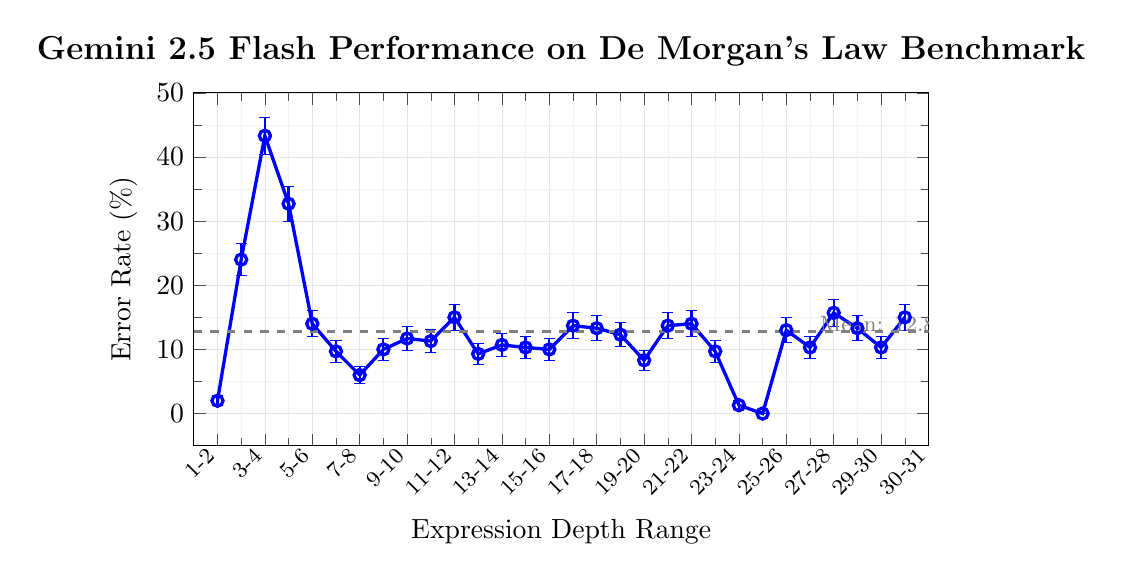
\begin{tikzpicture}
\begin{axis}[
    width=0.9\textwidth,
    height=0.5\textwidth,
    xlabel={Expression Depth Range},
    ylabel={Error Rate (\%)},
    xmin=0, xmax=31,
    ymin=-5, ymax=50,
    xtick={1,3,5,7,9,11,13,15,17,19,21,23,25,27,29,31},
    xticklabels={1-2,3-4,5-6,7-8,9-10,11-12,13-14,15-16,17-18,19-20,21-22,23-24,25-26,27-28,29-30,30-31},
    xticklabel style={rotate=45, anchor=east, font=\footnotesize},
    ytick={0,10,20,30,40,50},
    grid=both,
    minor tick num=1,
    grid style={line width=.1pt, draw=gray!10},
    major grid style={line width=.2pt,draw=gray!20},
    tick style={draw=black!70},
    xlabel style={font=\normalsize},
    ylabel style={font=\normalsize},
    title={Gemini 2.5 Flash Performance on De Morgan's Law Benchmark},
    title style={font=\large\bfseries},
]

% Main plot with error bars
\addplot[
    color=blue,
    line width=1.2pt,
    mark=o,
    mark size=2pt,
    error bars/.cd,
    y dir=both,
    y explicit,
    error bar style={line width=0.8pt},
] coordinates {
    (1, 2.0)   +- (0, 0.81)
    (2, 24.0)  +- (0, 2.47)
    (3, 43.3)  +- (0, 2.86)
    (4, 32.7)  +- (0, 2.71)
    (5, 14.0)  +- (0, 2.00)
    (6, 9.7)   +- (0, 1.71)
    (7, 6.0)   +- (0, 1.37)
    (8, 10.0)  +- (0, 1.73)
    (9, 11.7)  +- (0, 1.85)
    (10, 11.3) +- (0, 1.83)
    (11, 15.0) +- (0, 2.06)
    (12, 9.3)  +- (0, 1.68)
    (13, 10.7) +- (0, 1.79)
    (14, 10.3) +- (0, 1.76)
    (15, 10.0) +- (0, 1.73)
    (16, 13.7) +- (0, 1.99)
    (17, 13.3) +- (0, 1.96)
    (18, 12.3) +- (0, 1.90)
    (19, 8.3)  +- (0, 1.59)
    (20, 13.7) +- (0, 1.99)
    (21, 14.0) +- (0, 2.00)
    (22, 9.7)  +- (0, 1.71)
    (23, 1.3)  +- (0, 0.66)
    (24, 0.0)  +- (0, 0.0)
    (25, 13.0) +- (0, 1.94)
    (26, 10.3) +- (0, 1.76)
    (27, 15.7) +- (0, 2.10)
    (28, 13.3) +- (0, 1.96)
    (29, 10.3) +- (0, 1.76)
    (30, 15.0) +- (0, 2.06)
};

% Add horizontal line for mean
\addplot[
    color=gray,
    line width=0.8pt,
    dashed,
    no marks,
] coordinates {(0, 12.8) (31, 12.8)};
\node[anchor=west, font=\footnotesize, color=gray] at (axis cs:26,14) {Mean: 12.8\%};

\end{axis}
\end{tikzpicture}
\caption{Error rates with 95\% confidence intervals for logical expression simplification. 
Each point represents 300 evaluated samples. Error bars computed using binomial standard errors.}
\label{fig:error_rates_simple}
\end{figure}

\subsection{Qualitative Error Analysis}
An examination of specific failures reveals systematic flaws in the application of logical rules. The model often fails to correctly distribute negations across multiple nested clauses.

\begin{verbatim}
PROBLEM:
¬((¬(A0) ∧ ¬(A1)) ∨ ¬((¬(A2) ∧ ¬(A3))))

GROUND TRUTH (Canonical Form):
(A0 ∨ A1) ∧ (A2 ∨ A3)

LLM OUTPUT (Canonical Form):
(A0 ∨ A1) ∧ A2 ∧ A3

ANALYSIS:
The model correctly applied De Morgan's law to the first term,
transforming ¬(¬(A0) ∧ ¬(A1)) into (A0 ∨ A1). However, it failed on 
the second term, ¬(¬((¬(A2) ∧ ¬(A3)))), incorrectly simplifying 
it to an expression equivalent to A2 ∧ A3 instead of A2 ∨ A3.
\end{verbatim}

\section{Discussion}
The experimental results strongly support our central hypothesis. The non-zero error rate at `temperature=0` confirms that these failures are not artifacts of random sampling but are deterministic errors produced by the model's learned function. This indicates a fundamental failure of the model to generalize the principles of De Morgan's laws to novel combinations of operators, even after being prompted with examples.

The scaling of error rates with problem depth suggests the model is operating within a "combinatorial map fog." At low complexity (depth 1-2), the expressions may resemble patterns seen during training, allowing for successful interpolation. As complexity increases (depth 3-4), the model is pushed into sparser regions of the combinatorial state-space where its pattern-matching abilities break down, leading to a peak in errors at 43.3%. The subsequent behavior at higher depths (6+) is complex and non-monotonic, with error rates oscillating between roughly 8-16% rather than consistently decreasing. The surprising 0% error rate at depth 24-25 and continued volatility at depths 25-31 (ranging from 10.3% to 15.7%) challenges simple explanations and may suggest multiple competing failure modes or depth-dependent phase transitions in the model's processing strategy. The unexpected perfect performance at depth 24-25 (0% error rate) warrants further investigation. This anomaly, followed by a return to ~13% error rates, suggests that certain structural properties of expressions at specific depths may align with the model's learned representations in ways we do not yet understand. This finding contradicts any simple narrative of monotonic degradation or improvement with complexity.

Ultimately, these findings show that for tasks with vast combinatorial state-spaces, such as logical reasoning, relying on a model to learn the underlying principles from statistical patterns is inherently brittle. The model has not learned the algorithm of logical simplification; it has learned a statistical approximation that fails when pushed beyond the dense regions of its training data.

\section{Conclusion}
In this paper, we addressed the challenge of systematically measuring and understanding LLM hallucination. We introduced a symbolic benchmark using De Morgan's laws that creates a combinatorial landscape to test model generalization. Through experiments with a state-of-the-art LLM, we have shown that logical reasoning failures are systemic and deterministic, occurring even at zero temperature. The model's performance exhibits complex, non-monotonic patterns as problem depth increases, with a dramatic peak in errors at medium complexity (43.3% at depth 3-4) followed by volatile but generally lower error rates (8-16%) at higher depths, including an unexplained perfect performance at depth 24-25, confirming that hallucination can be a default behavior when pattern-matching fails. This work provides a concrete methodology for probing the limits of logical reasoning in LLMs and underscores the challenges that remain in building truly reliable and generalizable AI systems.

\bibliographystyle{plainnat}
\bibliography{references}

\end{document}
